\documentclass[border=15pt, multi, tikz]{standalone}
\usepackage{tikz}
\usepackage{amsmath,amssymb}
\usetikzlibrary{quotes,arrows.meta,positioning,3d,calc}

% ==============================================================================
%  HYALINE V2-D: ENHANCED EGNN LAYER DETAIL (3D Block Style)
% ==============================================================================

% --- Colors ---
\definecolor{inputCol}{HTML}{DAE8FC}
\definecolor{globalCol}{HTML}{B8D4E8}
\definecolor{edgeCol}{HTML}{D5E8D4}
\definecolor{msgCol}{HTML}{C8E6C9}
\definecolor{attnCol}{HTML}{E1D5E7}
\definecolor{nodeCol}{HTML}{DDA0DD}
\definecolor{coordCol}{HTML}{F8CECC}
\definecolor{injectCol}{HTML}{FFE6CC}
\definecolor{outputCol}{HTML}{D4EDDA}
\definecolor{edgeColor}{HTML}{666666}

% --- Connection Styles (NO ARROWHEADS) ---
\tikzstyle{connection}=[thick, draw=edgeColor]
\tikzstyle{inject}=[thick, draw=orange!70, densely dashed]
\tikzstyle{residual}=[thick, draw=edgeColor, densely dotted]

% --- BOX MACRO ---
% Corners:
%   a = top-left-front,     b = bottom-left-front
%   c = bottom-right-front, d = top-right-front
%   e = top-right-back,     f = bottom-right-back
%   g = bottom-left-back,   h = top-left-back

\tikzset{Box/.pic={\tikzset{/boxblock/.cd,#1}
        \tikzstyle{box}=[every edge/.append style={pic actions, densely dashed, opacity=.7},fill opacity=\opacity, pic actions,fill=\fill]
        \pgfmathsetmacro{\y}{\cubey*\scale}
        \pgfmathsetmacro{\z}{\cubez*\scale}
        \foreach[count=\i, evaluate=\i as \xlabel using {array({\boxlabels},\i-1)}, evaluate=\unscaledx as \k using {\unscaledx*\scale+\prev}, remember=\k as \prev (initially 0)] \unscaledx in \cubex {
            \pgfmathsetmacro{\x}{\unscaledx*\scale}
            \coordinate (a) at (\k-\x , \y/2 , \z/2);   % top-left-front
            \coordinate (b) at (\k-\x ,-\y/2 , \z/2);   % bottom-left-front
            \coordinate (c) at (\k    ,-\y/2 , \z/2);   % bottom-right-front
            \coordinate (d) at (\k    , \y/2 , \z/2);   % top-right-front
            \coordinate (e) at (\k    , \y/2 ,-\z/2);   % top-right-back
            \coordinate (f) at (\k    ,-\y/2 ,-\z/2);   % bottom-right-back
            \coordinate (g) at (\k-\x ,-\y/2 ,-\z/2);   % bottom-left-back
            \coordinate (h) at (\k-\x , \y/2 ,-\z/2);   % top-left-back
            \draw [box] (d) -- (a) -- (b) -- (c) -- cycle (d) -- (a) -- (h) -- (e) -- cycle;
            \path (b) edge ["\xlabel"',midway] (c);
            \xdef\LastEastx{\k} 
        }
        \draw [box] (d) -- (e) -- (f) -- (c) -- cycle;
        \path (b) edge ["\ylabel",midway] (a);
        % DIMENSION LABEL
        \tikzstyle{depthlabel}=[midway, sloped, below=1pt, font=\small]
        \path (c) edge ["\zlabel"',depthlabel] (f);
        % ANCHORS:
        % -east: CENTER of right face (where lines START - at face center)
        \coordinate (\name-east)  at ($(d)!0.5!(f)$);
        % -west/north/south: FRONT EDGE midpoints (where lines END - at boundary, no overlap)
        \coordinate (\name-west)  at ($(a)!0.5!(b)$);   % front-left edge
        \coordinate (\name-north) at ($(a)!0.5!(d)$);   % front-top edge
        \coordinate (\name-south) at ($(b)!0.5!(c)$);   % front-bottom edge
        % Caption anchor
        \coordinate (\name-caption) at ($(b)!0.5!(c) + (0,-1.5,0)$);
    },
    /boxblock/.search also={/tikz},
    /boxblock/.cd,
    width/.store in=\cubex, height/.store in=\cubey, depth/.store in=\cubez, scale/.store in=\scale,
    xlabel/.store in=\boxlabels, ylabel/.store in=\ylabel, zlabel/.store in=\zlabel,
    name/.store in=\name, fill/.store in=\fill, opacity/.store in=\opacity,
    fill={inputCol}, opacity=0.7, width=2, height=13, depth=15, scale=.2,
    xlabel={{"",""}}, ylabel=, zlabel=, name=,
}

\begin{document}
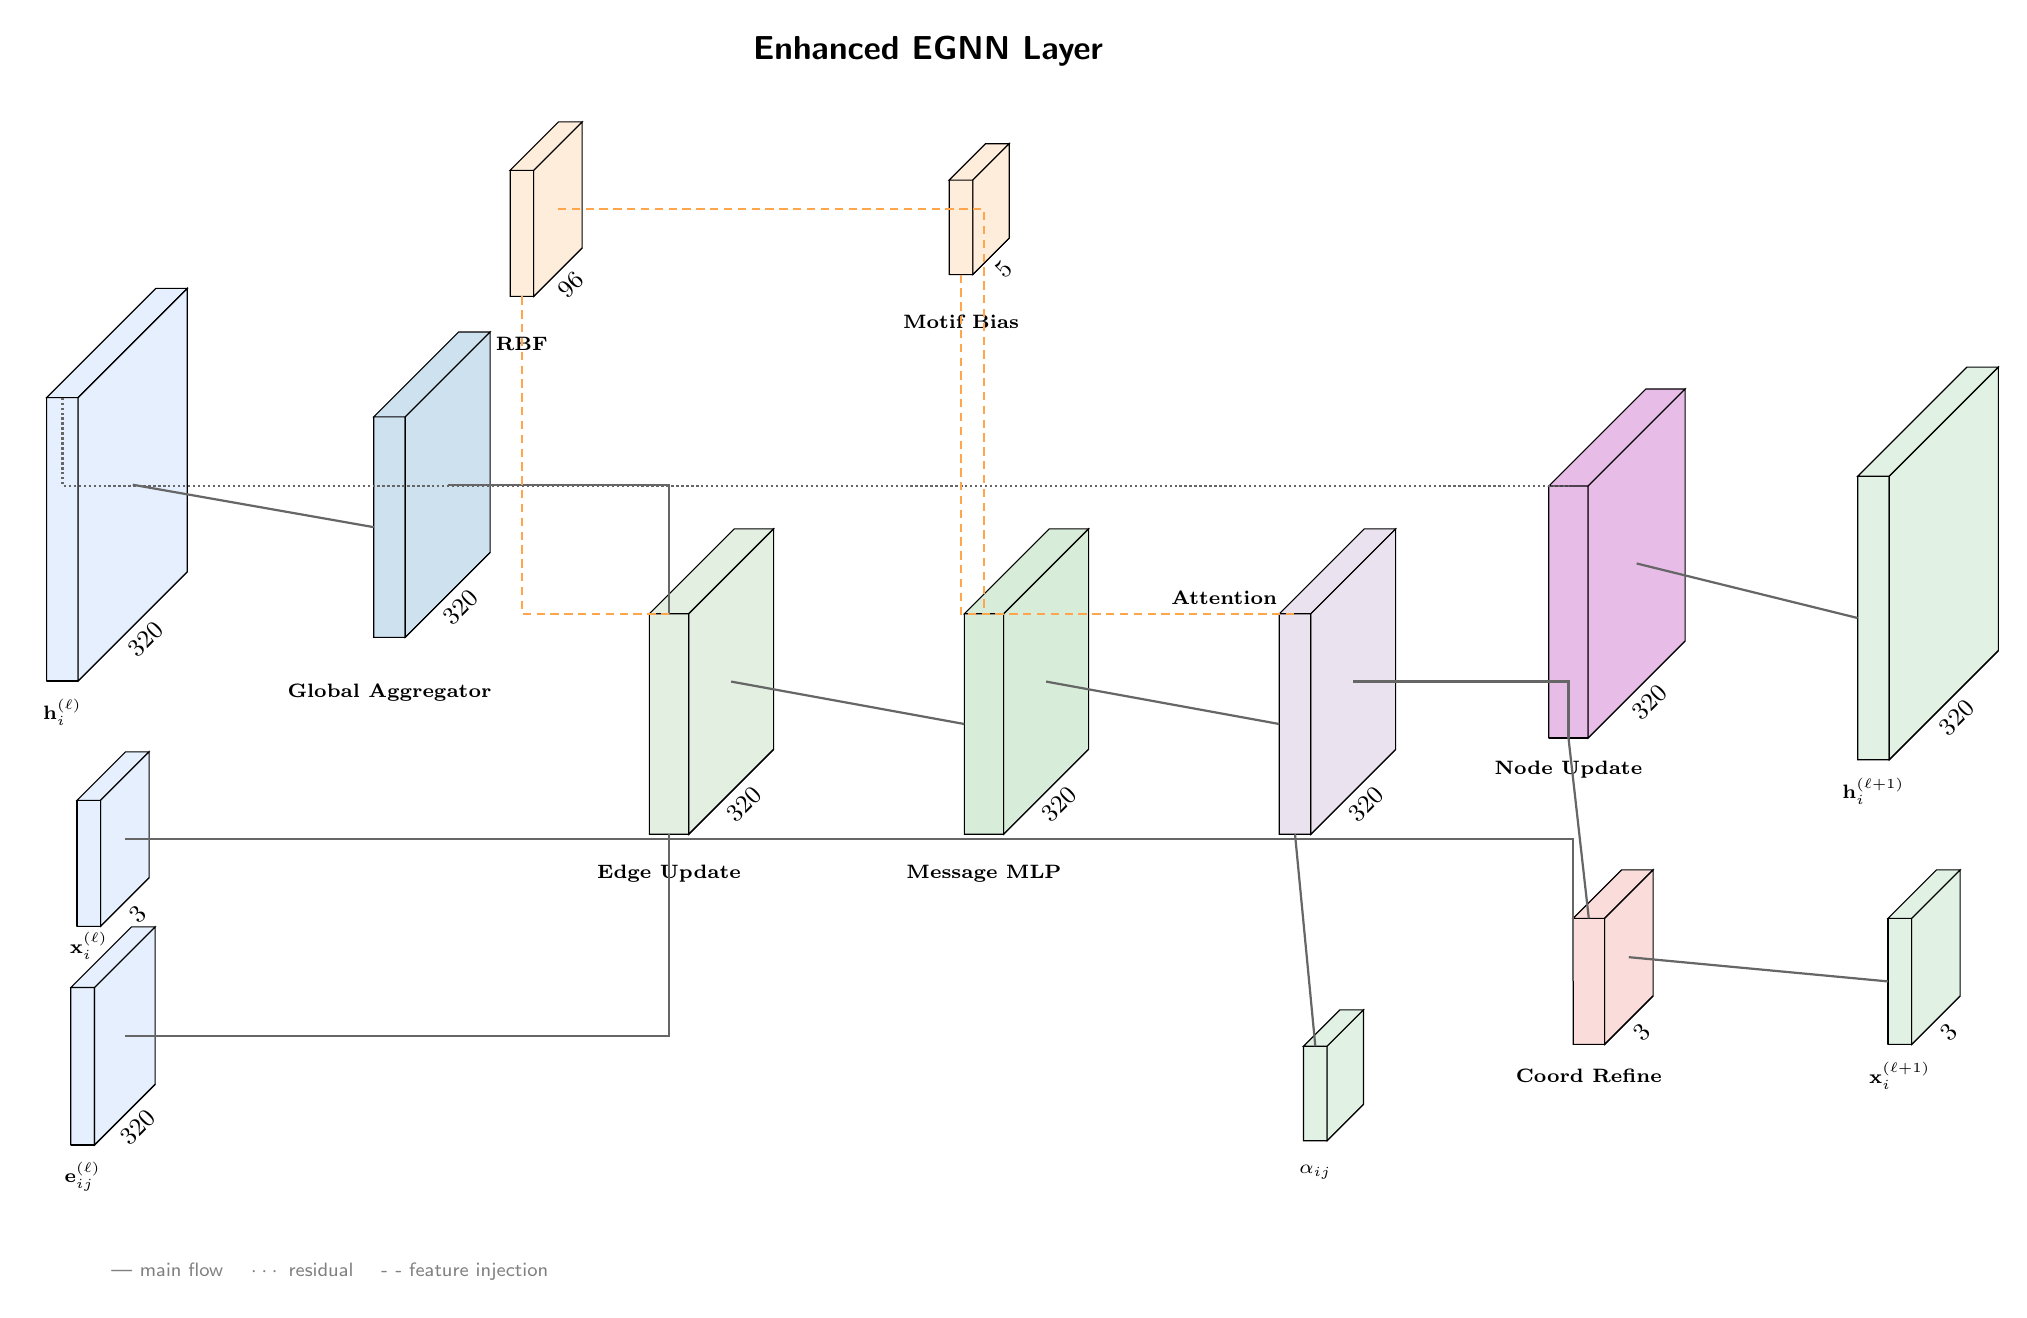
\begin{tikzpicture}

    % ==== TITLE ====
    \node[font=\sffamily\bfseries\large] at (10.5, 7) {Enhanced EGNN Layer};

    % === INPUT FEATURES ===
    \pic[shift={(0, 1.5, 0)}] at (0,0,0) 
        {Box={name=h_in, fill=inputCol, opacity=0.7, height=18, width=2, depth=18, zlabel=320}};
    \node[font=\scriptsize\bfseries] at ($(h_in-caption) + (0, 1.1, 0)$) {$\mathbf{h}_i^{(\ell)}$};
    
    \pic[shift={(0, -3, 0)}] at (0,0,0) 
        {Box={name=x_in, fill=inputCol, opacity=0.7, height=8, width=1.5, depth=8, zlabel=3}};
    \node[font=\scriptsize\bfseries] at ($(x_in-caption) + (0, 1.25, 0)$) {$\mathbf{x}_i^{(\ell)}$};
    
    \pic[shift={(0, -5.5, 0)}] at (0,0,0) 
        {Box={name=e_in, fill=inputCol, opacity=0.7, height=10, width=1.5, depth=10, zlabel=320}};
    \node[font=\scriptsize\bfseries] at ($(e_in-caption) + (0, 1.1, 0)$) {$\mathbf{e}_{ij}^{(\ell)}$};

    % === INJECTED FEATURES ===
    \pic[shift={(5.5, 5, 0)}] at (0,0,0) 
        {Box={name=rbf, fill=injectCol, opacity=0.7, height=8, width=1.5, depth=8, zlabel=96}};
    \node[font=\scriptsize\bfseries] at ($(rbf-caption) + (0, 0.9, 0)$) {RBF};
    
    \pic[shift={(11, 5, 0)}] at (0,0,0) 
        {Box={name=motif, fill=injectCol, opacity=0.7, height=6, width=1.5, depth=6, zlabel=5}};
    \node[font=\scriptsize\bfseries] at ($(motif-caption) + (0, 0.9, 0)$) {Motif Bias};

    % === PROCESSING BLOCKS ===
    \pic[shift={(4, 1.5, 0)}] at (0,0,0) 
        {Box={name=global, fill=globalCol, opacity=0.7, height=14, width=2, depth=14, zlabel=320}};
    \node[font=\scriptsize\bfseries] at ($(global-caption) + (0, 0.8, 0)$) {Global Aggregator};
    
    \pic[shift={(7.5, -1, 0)}] at (0,0,0) 
        {Box={name=edgeupd, fill=edgeCol, opacity=0.7, height=14, width=2.5, depth=14, zlabel=320}};
    \node[font=\scriptsize\bfseries] at ($(edgeupd-caption) + (0, 1, 0)$) {Edge Update};
    
    \pic[shift={(11.5, -1, 0)}] at (0,0,0) 
        {Box={name=msg, fill=msgCol, opacity=0.7, height=14, width=2.5, depth=14, zlabel=320}};
    \node[font=\scriptsize\bfseries] at ($(msg-caption) + (0, 1, 0)$) {Message MLP};
    
    \pic[shift={(15.5, -1, 0)}] at (0,0,0) 
        {Box={name=attn, fill=attnCol, opacity=0.7, height=14, width=2, depth=14, zlabel=320}};
    \node[font=\scriptsize\bfseries] at ($(attn-caption) + (-0.9, 4.5, 0)$) {Attention};
    
    \pic[shift={(19, 0.5, 0)}] at (0,0,0) 
        {Box={name=nodeupd, fill=nodeCol, opacity=0.7, height=16, width=2.5, depth=16, zlabel=320}};
    \node[font=\scriptsize\bfseries] at ($(nodeupd-caption) + (0, 1.1, 0)$) {Node Update};
    
    \pic[shift={(19, -4.5, 0)}] at (0,0,0) 
        {Box={name=coord, fill=coordCol, opacity=0.7, height=8, width=2, depth=8, zlabel=3}};
    \node[font=\scriptsize\bfseries] at ($(coord-caption) + (0, 1.1, 0)$) {Coord Refine};

    % === OUTPUT FEATURES ===
    \pic[shift={(23, 0.5, 0)}] at (0,0,0) 
        {Box={name=h_out, fill=outputCol, opacity=0.7, height=18, width=2, depth=18, zlabel=320}};
    \node[font=\scriptsize\bfseries] at ($(h_out-caption) + (0, 1.1, 0)$) {$\mathbf{h}_i^{(\ell+1)}$};
    
    \pic[shift={(23, -4.5, 0)}] at (0,0,0) 
        {Box={name=x_out, fill=outputCol, opacity=0.7, height=8, width=1.5, depth=8, zlabel=3}};
    \node[font=\scriptsize\bfseries] at ($(x_out-caption) + (0, 1.1, 0)$) {$\mathbf{x}_i^{(\ell+1)}$};
    
    \pic[shift={(15.5, -6, 0)}] at (0,0,0) 
        {Box={name=attn_out, fill=outputCol, opacity=0.7, height=6, width=1.5, depth=6}};
    \node[font=\scriptsize\bfseries] at ($(attn_out-caption) + (0, 1.1, 0)$) {$\alpha_{ij}$};


    % ==== CONNECTIONS ====
    % -east: starts from face center (good)
    % -west/north/south: ends at front edge (no overlap)
    
    % h_in -> Global
    \draw[connection] (h_in-east) -- (global-west);
    
    % Global -> Edge Update
    \draw[connection] (global-east) -| (edgeupd-north);
    
    % e_in -> Edge Update
    \draw[connection] (e_in-east) -| (edgeupd-south);
    
    % Edge Update -> Message
    \draw[connection] (edgeupd-east) -- (msg-west);
    
    % Message -> Attention
    \draw[connection] (msg-east) -- (attn-west);
    
    % Attention -> Node Update
    \draw[connection] (attn-east) -| (nodeupd-south);
    
    % Residual: h_in to Node Update
    \draw[residual] (h_in-north) |- (nodeupd-north);
    
    % Node Update -> h_out
    \draw[connection] (nodeupd-east) -- (h_out-west);
    
    % Node Update -> Coord Refine
    \draw[connection] (nodeupd-south) -- (coord-north);
    
    % x_in -> Coord Refine
    \draw[connection] (x_in-east) -| (coord-west);
    
    % Coord Refine -> x_out
    \draw[connection] (coord-east) -- (x_out-west);
    
    % Attention -> attn_out
    \draw[connection] (attn-south) -- (attn_out-north);
    
    % === INJECTION ===
    \draw[inject] (rbf-south) |- (edgeupd-north);
    \draw[inject] (rbf-east) -| (msg-north);
    \draw[inject] (motif-south) |- (attn-north);
    
    % ==== LEGEND ====
    \node[font=\sffamily\scriptsize, text=gray, anchor=west] at (0, -8.5) {
        \textbf{---} main flow \quad \textbf{$\cdots$} residual \quad \textbf{- -} feature injection
    };

\end{tikzpicture}
\end{document}